\documentclass[a4paper,10pt]{article}
\usepackage[T1]{fontenc}
\usepackage[utf8]{inputenc}
\usepackage[english]{babel}
\usepackage{lmodern}
\usepackage[top=1.6cm,bottom=1.8cm,left=1.9cm,right=1.9cm]{geometry}
\usepackage{titlesec,enumitem,xcolor,graphicx,lastpage,fancyhdr}
\usepackage{fontawesome5}
\usepackage[hidelinks]{hyperref}

\hypersetup{colorlinks=true,urlcolor=blue!70!black,linkcolor=blue!70!black}
\pagestyle{fancy}\fancyhf{}\renewcommand{\headrulewidth}{0pt}
\fancyfoot[C]{\small\color{gray}Page \thepage\ of \pageref{LastPage}}
\setlength{\parindent}{0pt}

\titleformat{\section}{\large\bfseries\color{blue!70!black}}{}{0em}{}[\vspace{-0.7em}\rule{\textwidth}{0.5pt}]
\titlespacing{\section}{0pt}{9pt}{5pt}
\setlist[itemize]{leftmargin=1.1em,itemsep=2pt,topsep=2pt,parsep=0pt}
\newcommand{\role}[4]{\vspace{3pt}\noindent\hspace{0.6em}\parbox[t]{0.38\textwidth}{\raggedright\textbf{#1}}\hfill\parbox[t]{0.58\textwidth}{\raggedleft\textit{#2}}\\{\textit{#3}\hfill\textit{#4}}\vspace{1pt}}

\begin{document}
\noindent
\begin{minipage}[t]{0.78\textwidth}
\vspace{0pt}
{\huge\bfseries Prabhavit Gupta}\\[8pt]
{\small \faPhone\ +39-351-610-7807 \quad \faEnvelope\ \href{mailto:prabhavitg@gmail.com}{prabhavitg@gmail.com} \quad \faLinkedin\ \href{https://www.linkedin.com/in/prabhavit/}{Linkedin} \quad \faMapMarker*\ Venice, Italy}
\end{minipage}\hfill
\begin{minipage}[t]{0.18\textwidth}
\vspace{0pt}\raggedleft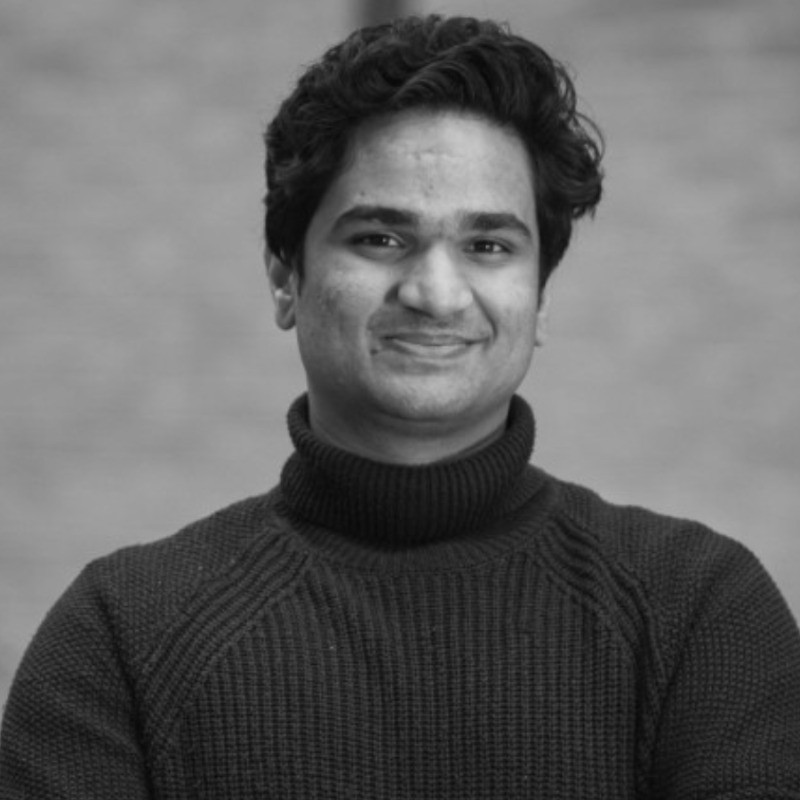
\includegraphics[width=2.3cm,height=2.3cm,keepaspectratio]{photo.jpg}
\end{minipage}

\section{Career Summary}
\begin{itemize}
\item AI Technical Lead \& Solutions Architect with deep expertise in AI-assisted software engineering, Generative AI integration, and production agentic architectures.
\item Proven leader in establishing AI engineering standards, mentoring developers on LLM tooling (Cursor, Claude, Copilot), and delivering scalable RAG/agent solutions.
\item Expert in orchestrating LLM APIs, vector stores, Model Context Protocol (MCP), and microservices with rigorous governance, security, and automated evaluation frameworks.
\end{itemize}

\section{Technical Skills}
\begin{itemize}
\item \textbf{Generative AI \& Agents} -- LLMs, AI Agents, MCP (Model Context Protocol), LangChain, LlamaIndex, RAG Pipelines, Vector DBs (pgvector, Pinecone)
\item \textbf{AI-Assisted Engineering} -- Claude Code, Cursor, GitHub Copilot, Prompt Optimization, Context Engineering, Automated Code Generation
\item \textbf{Software Architecture} -- Python, TypeScript, REST APIs, Microservices, Event-Driven Architecture, Docker, CI/CD, Automated Testing
\item \textbf{Cloud \& Governance} -- AWS, Azure AI, GCP, AI Governance, Data Privacy, Access Controls, Observability \& Telemetry
\end{itemize}

\section{Visa \& Language}
\begin{itemize}
\item \textbf{Language} -- English (Professional / Fluent), Italian (Conversational / Intermediate), Hindi (Native)
\item \textbf{Work Authorization} -- European Long Term Residence Permit - No Sponsorship required.
\end{itemize}

\section{Professional Experience}
\role{\href{https://flowspace.co}{FlowSpace.co}}{Technical Lead \& AI Architect (Full time, Freelance)}{London, UK}{Mar 2024 -- Ongoing}
\begin{itemize}
\item \textbf{AI Technical Direction \& Architecture:}
\begin{itemize}[label=--]
\item Spearheaded technical direction for enterprise platform adoption of AI-assisted engineering, standardizing Cursor and Claude workflows across team.
\item Architected autonomous customer service and scheduling AI agents integrated with external booking APIs (Office Rnd, Nexudus) via MCP and webhooks.
\item Built production RAG infrastructure utilizing embedding pipelines, semantic search, and prompt caching to reduce token overhead by 45\%.
\item Enforced strict AI governance protocols including input sanitization, automated regression testing, and hallucination guardrails.
\end{itemize}
\item \textbf{Engineering Leadership \& Scale:}
\begin{itemize}[label=--]
\item Guided and mentored distributed engineering teams on modern cloud architectures, API contract design, and test-driven development.
\item Scaled platform from 2,000 to 4,500+ active users with 99.9\% uptime across production AI microservices.
\end{itemize}
\item \textit{Tools: Python, TypeScript, MCP, Next.js, FastAPI, pgvector, Docker, GitHub Actions, AWS}
\end{itemize}

\role{Urlink}{Senior AI Solutions Engineer}{Milan, Italy}{Jul 2023 -- Feb 2024}
\begin{itemize}
\item Led architecture of automated document analysis and intelligent entity extraction microservices for enterprise clients.
\item Implemented semantic search engines using embeddings and vector indexing, improving query retrieval accuracy by 30\%.
\item Designed robust CI/CD deployment pipelines incorporating automated linting, test suites, and model evaluation benchmarks.
\end{itemize}

\role{UltraStrategy}{Automation \& AI Developer}{Remote, Germany}{Sep 2022 -- Jun 2023}
\begin{itemize}
\item Developed modular integration middleware connecting enterprise analytics tools via RESTful endpoints and secure token exchange.
\item Automated ETL data pipelines across cloud endpoints, validating payload integrity and enforcing schema validation.
\end{itemize}

\section{Education}
\role{Politecnico di Milano}{M.Sc. in Management Engineering (Digital Business \& ICT)}{Milan, Italy}{2020 -- 2023}
\role{Thapar Institute of Engineering and Technology}{B.E. in Mechanical Engineering}{Punjab, India}{2014 -- 2018}

\end{document}
